\documentclass{standalone}
\usepackage{tikz}
\usepackage{ctex,siunitx}
\setCJKmainfont{Noto Serif CJK SC}
\usepackage{tkz-euclide}
\usepackage{amsmath}
\usepackage{wasysym}
\usetikzlibrary{patterns, calc}
\usetikzlibrary {decorations.pathmorphing, decorations.pathreplacing, decorations.shapes,}
\begin{document}
\small
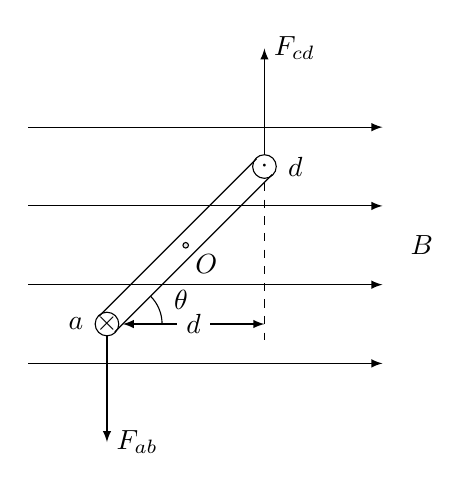
\begin{tikzpicture}[>=latex,scale=1]
  \foreach \x in {-1,0,1,2}
  {
    \draw[->](-1.5,\x)--(3,\x);
  }
  \node at (3.5,.5){$B$};
  \draw[->](1.5,1.5)--(1.5,3)node[right]{$F_{cd}$};
  \draw[->](-.5,-.5)--(-.5,-2)node[right]{$F_{ab}$};
  \draw[dashed](1.5,1.5)--(1.5,-.7);
  \draw[<->](-.3,-.5)--node[fill=white]{$d$}(1.5,-.5);
  \draw[fill=white](1.5,1.5)node{$\cdot$} circle(.15); 
  \draw[fill=white](-.5,-.5)node{$\times$} circle(.15); 
  \draw(1.5-.1,1.5+.1)--(-.5-.1,-.5+.1);
  \draw(1.5+.1,1.5-.1)--(-.5+.1,-.5-.1);
  \node at (1.5,1.5)[right=5pt]{$d$};
  \node at (-.5,-.5)[left=5pt]{$a$};
  \tkzDefPoints{.5/.5/O, 1.5/-.5/A, -.3/-.5/B, 1.6/1.4/O'}
  \tkzDrawPoints(O)
  \tkzLabelPoints[below right](O)
  \tkzLabelAngle[pos=.8](A,B,O'){$\theta$}
  \tkzMarkAngles[mark=none, size=.5](A,B,O')
\end{tikzpicture}
\end{document}